\documentclass[xcolor=table,aspectratio=169]{beamer}
\usepackage{beamerthemesplit}
\usepackage{wrapfig}
\usetheme{SPbGU}
\usepackage{pdfpages}
\usepackage{amsmath}
\usepackage{cmap}
\usepackage[T2A]{fontenc}
\usepackage[utf8]{inputenc}
\usepackage[english]{babel}
\usepackage{indentfirst}
\usepackage{mathtools}
\usepackage{pgf}
\usepackage{soul}
\usepackage{tikz}
\usepackage{multirow}
\usepackage[noend]{algpseudocode}
\usepackage{algorithm}
\usepackage{algorithmicx}
\usepackage{fancyvrb}

\usepackage{minted}

\usetikzlibrary{shapes, arrows, automata, fit, calc, positioning}


\usepackage{fontawesome}

\usetikzlibrary{shapes.callouts}

\usepackage{xparse}

%for [[ ]]
\usepackage{stmaryrd}


\tikzset{
    invisible/.style={opacity=0,text opacity=0},
    visible on/.style={alt=#1{}{invisible}},
    alt/.code args={<#1>#2#3}{%
      \alt<#1>{\pgfkeysalso{#2}}{\pgfkeysalso{#3}} % \pgfkeysalso doesn't change the path
    },
}

\NewDocumentCommand{\mycallout}{r<> O{opacity=0.8,text opacity=1} m m m}{%
\tikz[remember picture, overlay]\node[align=center, fill=cyan!20, text width=#5cm,
#2,visible on=<#1>, rounded corners,
draw,rectangle callout,anchor=pointer,callout relative pointer={(230:1cm)}]
at (#3) {#4};
}

%\newcommand{\tikzmark}[1]{\tikz[overlay,remember picture,baseline=-0.5ex] \node (#1) {};}



\usepackage{tabularx}
\newcolumntype{Y}{>{\raggedleft\arraybackslash}X}

\renewcommand{\thealgorithm}{}

\newtheorem{mytheorem}{Theorem}
\renewcommand{\thealgorithm}{}

\newcommand{\tikzmark}[1]{\tikz[overlay,remember picture] \node (#1) {};}
\def\Put(#1,#2)#3{\leavevmode\makebox(0,0){\put(#1,#2){#3}}}

\newcommand{\ltz}{$< 1$}

\newcommand{\nodeDistanceRsm}{2.5cm}
\newcommand{\rsmInnerXSep}{0.1cm}
\newcommand{\rsmInnerYSep}{0.8cm}

\tikzset{
    state/.style={
           rectangle,
           rounded corners,
           draw=black, very thick,
           minimum height=2em,
           inner sep=2pt,
           text centered,
           },
}

\makeatletter
\AtBeginEnvironment{minted}{\dontdofcolorbox}
\def\dontdofcolorbox{\renewcommand\fcolorbox[4][]{##4}}
\makeatother

\beamertemplatenavigationsymbolsempty

\title[GLL-based CFPQ for Neo4j]{GLL-based Context-Free Path Querying for Neo4j}
%\subtitle[YaccConstructor]{Parsing techniques for graph analysis}
\institute[SPbSU]{
Saint Petersburg State University
}


\author[Semyon Grigorev]{Vadim Abzalov, Vlada Pogozhelskaya, Vladimir Kutuev, \\ Olga Bachishche, \textbf{Semyon Grigorev}}

\date{October 31, 2025}

\begin{document}
{
\begin{frame}[fragile]
  \begin{table}
  \centering
  \begin{tabularx}{\linewidth}{XcX}
    
\includegraphics[height=1.5cm]{pictures/damdid_logo.png} \hfill
    & \hfill %\begin{minipage}[t]{0.3\textwidth}\center \includegraphics[height=1.5cm]{pictures/EDBT.png} \hfill
      %\end{minipage}
    & \hfill 
\includegraphics[height=1.5cm]{pictures/SPbGU_Logo.png}
  \end{tabularx}
  \end{table}
  \titlepage
\end{frame}
}

\begin{frame}[fragile] \frametitle{Formal Language Constrained Path Querying}
      \begin{minipage}[m]{0.45\linewidth}
  \raisebox{-0.5\totalheight}{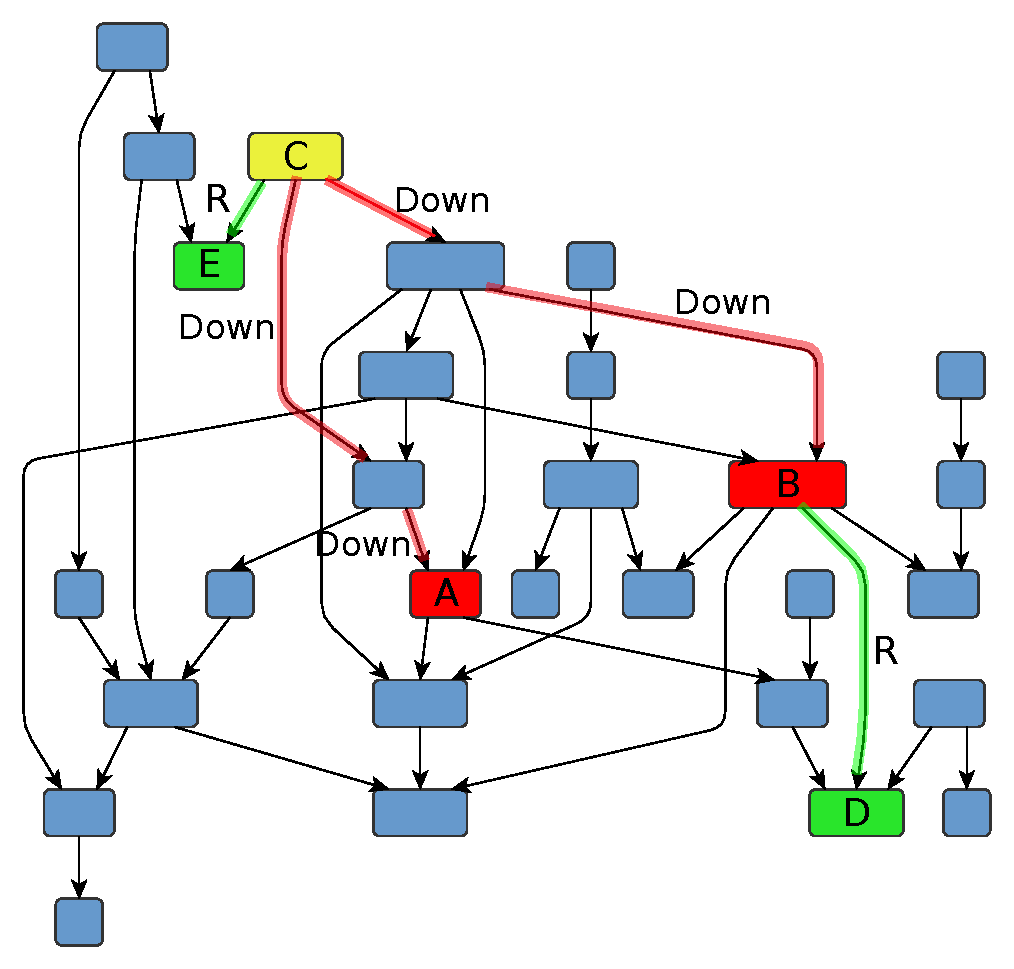
\includegraphics[width=\textwidth]{pictures/hierarchical_rpq.pdf}}
  \end{minipage}\hfill
  \begin{minipage}[m]{0.5\linewidth}
  Navigation through an edge-labeled graph

  \vfill

  \begin{itemize}
        \item \textbf{Path} specifies a \textbf{word} formed by the~labels of the edges
        \item \textbf{Paths constraint} is a \textbf{language}: the~word specified by the path should be in~the given language
        \item The expressiveness of constraints is related~to \textbf{formal languages classes}
  \end{itemize}
  \end{minipage}

\end{frame}


\begin{frame}[fragile] \frametitle{Regular Path Queries (RPQ)}
      \begin{minipage}[m]{0.45\linewidth}
  \raisebox{-0.5\totalheight}{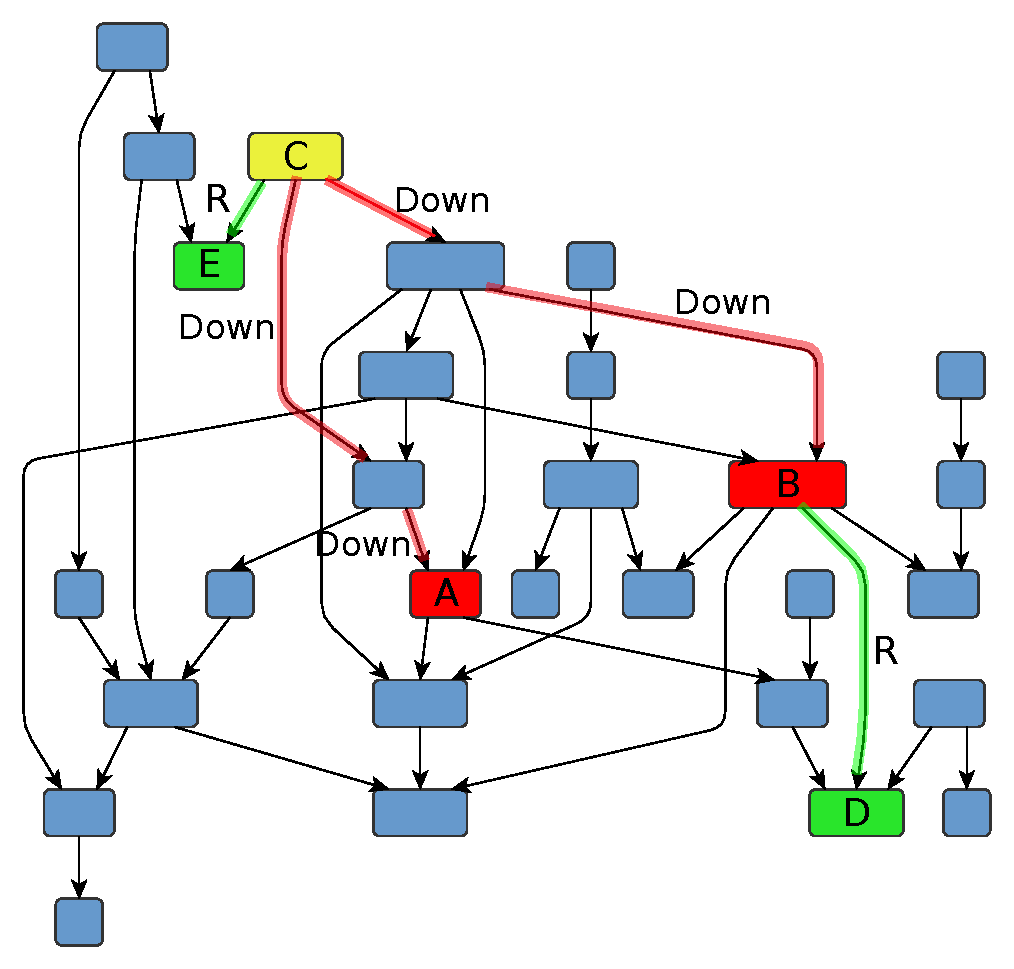
\includegraphics[width=\textwidth]{pictures/hierarchical_rpq.pdf}}
  \end{minipage}\hfill
  \begin{minipage}[m]{0.5\linewidth}
  \textbf{Regular} languages as constraints

  \vfill


  \begin{itemize}
        \item Which nodes are reachable from \textbf{C} by arbitrary number of $\textbf{R} \text{ and } \textbf{Down}$ edges?
        \item Regular language $\mathcal{L} = (\textit{R} \mid \textit{Down})^*$
  \end{itemize}
  \vspace{2cm}
  \begin{itemize}    
    \item Part of GQL and SQL/PGQ (ISO/IEC 9075-16:2023)
  \end{itemize}

  \end{minipage}

\end{frame}


\begin{frame}[fragile] \frametitle{Context-Free Path Queries (CFPQ)}
      \begin{minipage}[m]{0.45\linewidth}
  \raisebox{-0.5\totalheight}{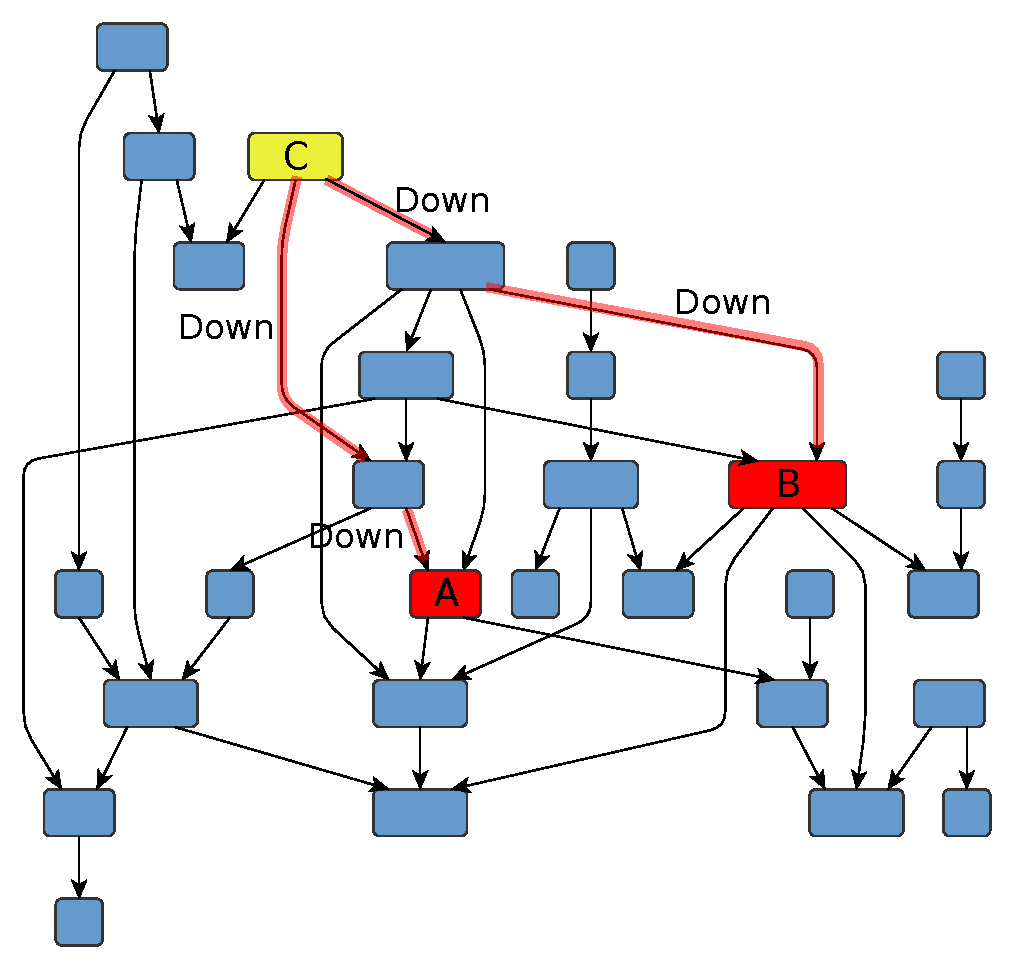
\includegraphics[width=\textwidth]{pictures/hierarchical.pdf}}
  \end{minipage}\hfill
  \begin{minipage}[m]{0.5\linewidth}
  \textbf{Context-free} languages as constraints
  \begin{itemize}
        \item Are nodes A and B on the same level of hierarchy?
        \item Is there a path of form $\overline{\textbf{Down}}^n \, \textbf{Down}^n$ between A and B?
        \item Context-free grammar: $\textit{SameLvl} \to \overline{\textit{Down}} \ \textit{SameLvl} \ \textit{Down} \mid \varepsilon$
  \end{itemize}
  \pause

  \vspace{0.3cm}


  Applications
    \begin{itemize}
      \item Static code analysis [\href{https://dl.acm.org/doi/10.1145/199448.199462}{T. Reps, et al, 1995}]
      \item Graph segmentation [\href{https://dblp.org/rec/conf/icde/0001D19.html}{H. Miao, et al, 2019}]
      \item Bio data analysis [\href{https://pubmed.ncbi.nlm.nih.gov/20134073/}{P. Sevon, et al, 2008}]
      \item \ldots
    \end{itemize}

  \end{minipage}

  \end{frame}

\begin{frame}[fragile] \frametitle{Problem Statement}
   \begin{itemize}
      \item J. Kuijpers, et al\footnote<.(1)->{Jochem Kuijpers, George Fletcher, Nikolay Yakovets, and Tobias Lindaaker. 2019. An Experimental Study of Context-Free Path Query Evaluation Methods.}: existing algorithms are too slow to be used in practical applications (in~the context of Neo4j)      
      \item Reachability in the focus
      \begin{itemize}
        \item Paths needed in some applications
        \item Not for all pairs, but for specified start vertices
      \end{itemize}
      \vfill
      \item[\faQuestion] How to create faster multiple source context-free all paths querying algorithm?
    \end{itemize}

\end{frame}


\begin{frame}[fragile] \frametitle{Proposed Solution}
  \begin{itemize}
      \item \textbf{Generalized LL (GLL)}\footnote{A. Afroozeh, Anastasia Izmaylova. Faster, Practical GLL Parsing. 2015} as a base
      \begin{itemize}
        \item Arbitrary grammars (including left-recursive and ambiguous) without transformations
        \item \textbf{Shared Packed Parse Forest (SPPF)} is a native representation of all paths
        \item Directed --- native support of source vertices
      \end{itemize}
      \item \textbf{Recursive State Machine (RSM)} to represent constraints
      \begin{itemize}
        \item Instead of grammar in (E)BNF
      \end{itemize}
  \end{itemize}

\end{frame}

\begin{frame}[fragile] \frametitle{Generalized LL for CFPQ: The Idea}
  \begin{center}
      \includegraphics[width=0.99\textwidth]{pictures/gll.pdf}
  \end{center}
\end{frame}

\begin{frame}[fragile] \frametitle{SPPF is a Representation of All Paths of Interest}
  \begin{center}
      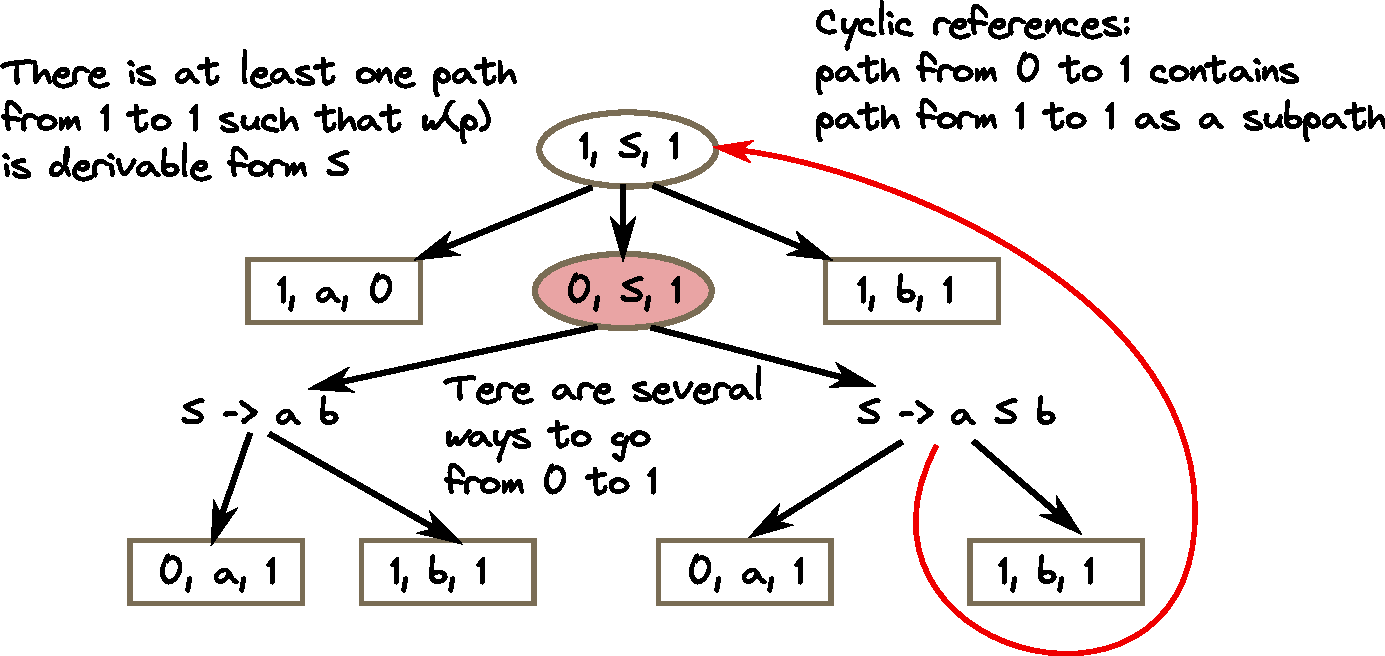
\includegraphics[width=0.89\textwidth]{pictures/sppf.pdf}
  \end{center}
\end{frame}


\begin{frame}[fragile] \frametitle{Trees And Paths}
  \begin{center}
      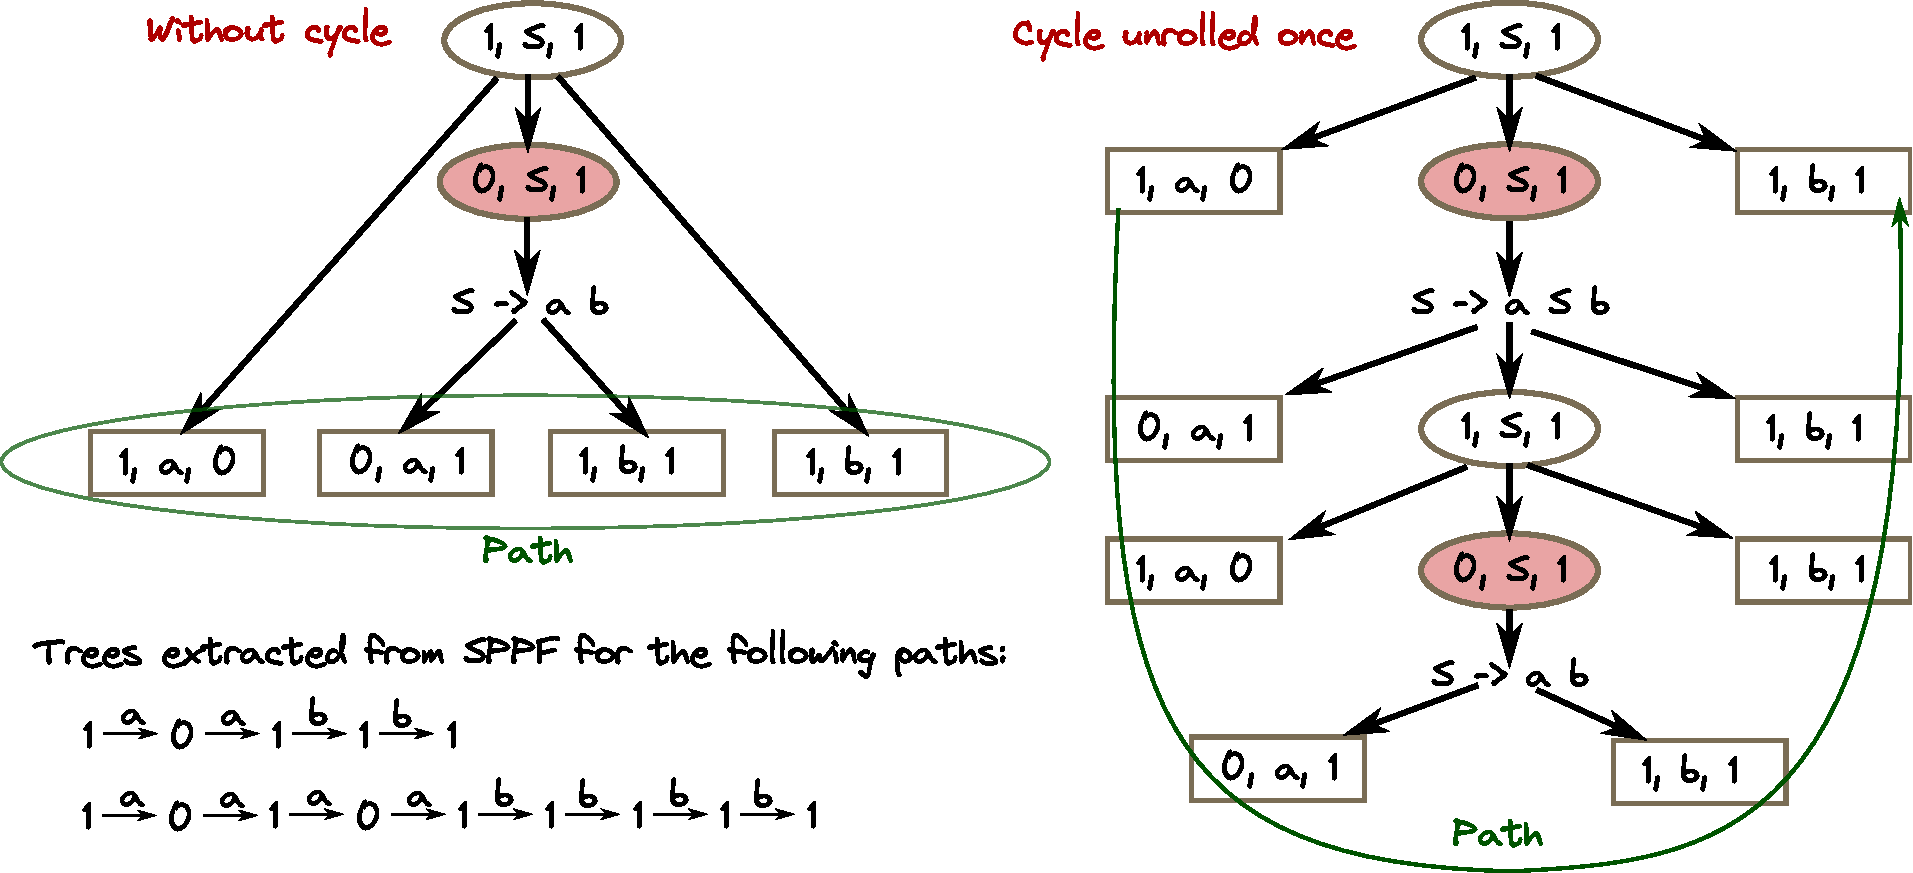
\includegraphics[width=0.99\textwidth]{pictures/Trees.pdf}
  \end{center}
\end{frame}


\begin{frame}[fragile] \frametitle{Context-Free Languages Are Closed Under Intersection With Regular Ones}
  \begin{center}
      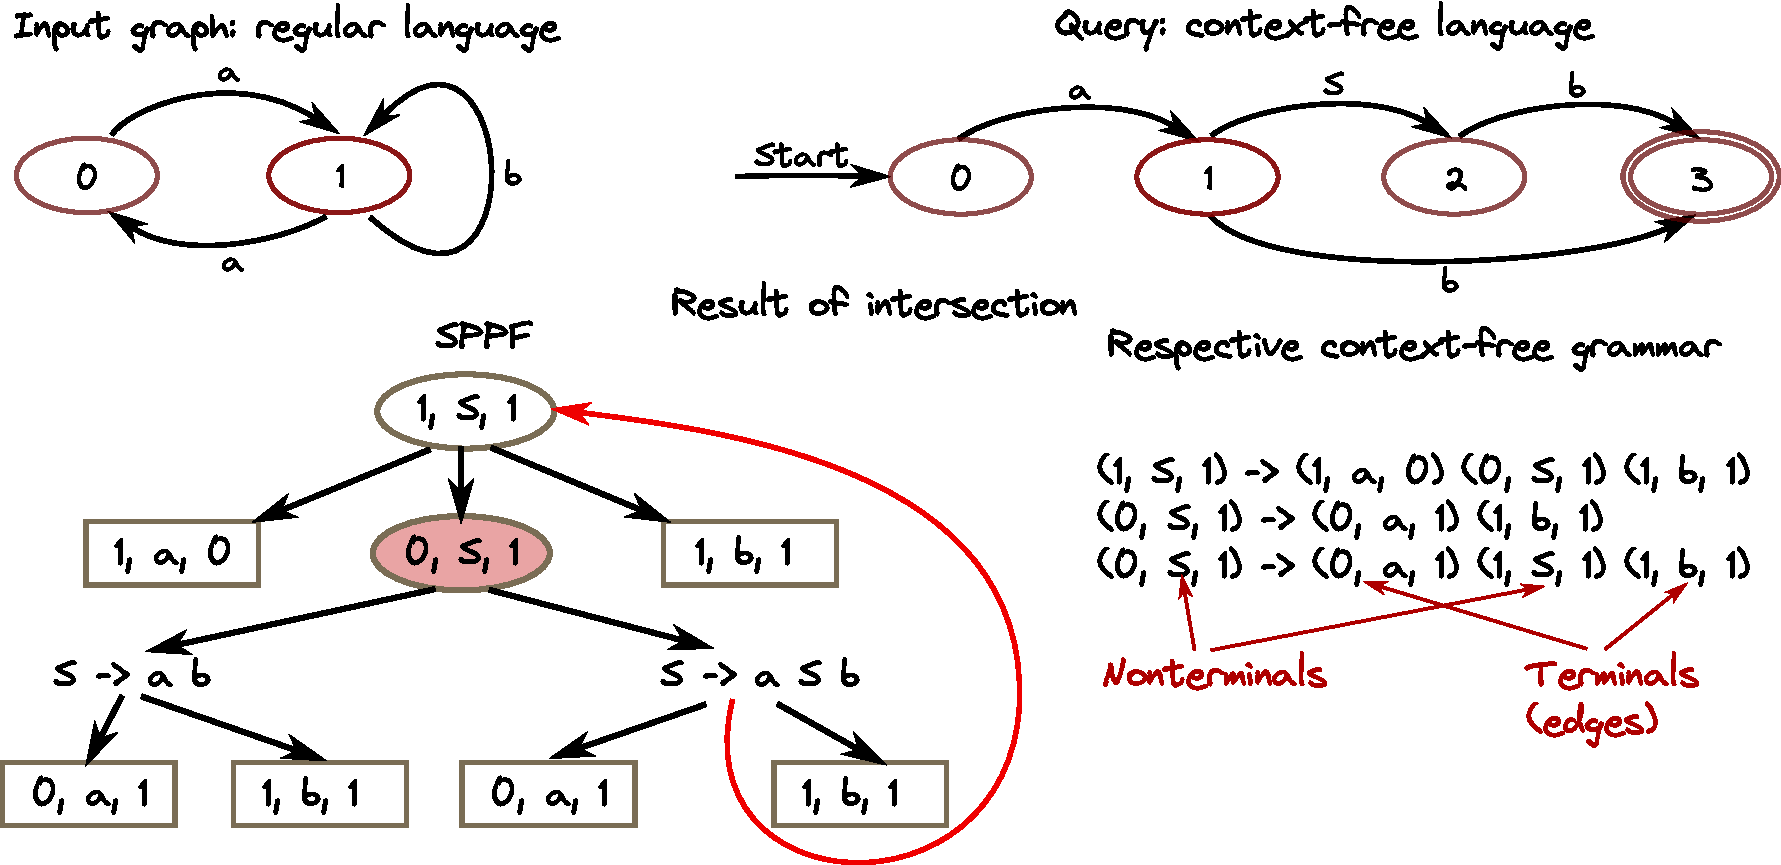
\includegraphics[width=0.99\textwidth]{pictures/Intersection.pdf}
  \end{center}
\end{frame}


%\begin{frame}[fragile] \frametitle{Recursive State Machine}  
%\begin{tikzpicture}[thick,scale=1.0, node distance=\nodeDistanceRsm,
%                    shorten >=1pt,on grid,auto] 
%
%  \node[state, initial left] (q_0)   {$q_0$};
%  \node[state] (q_1) [above right=of q_0] {$q_1$};
%  \node[state] (q_2) [right=of q_1] {$q_2$};
%  \node[state, accepting] (q_3) [below right=of q_2] {$q_3$};
%  \node[state] (q_4) [below right=of q_0] {$q_4$};
%  \node[state] (q_5) [right=of q_4] {$q_5$};
%
%  \node[draw=black, fit=(q_0) (q_1) (q_5) (q_3), inner xsep=0.1cm, inner ysep=0.1cm] (E) {};
%  \node[below right] at (E.north west) {S};
%
%  \path[->]
%    (q_0) edge[sloped, right, above, bend left] node {$\overline{subClassOf}$} (q_1)
%    (q_1) edge node {$q_0$} (q_2)
%    (q_2) edge[sloped, right, above, bend left] node {$subClassOf$} (q_3)
%    (q_1) edge[sloped, above] node {$subClassOf$} (q_3)
%    (q_0) edge[bend right, sloped, below] node {$\overline{type}$} (q_4)
%    (q_4) edge[below] node {$q_0$} (q_5)
%    (q_5) edge[left, sloped, bend right, below] node {$type$} (q_3)
%    (q_4) edge[sloped, above] node {$type$} (q_3);
%\end{tikzpicture}
%\end{frame}




\begin{frame}[fragile] \frametitle{Implementation Details}
  \begin{itemize}
  \item !!!
  \item !!!
  \item !!!
  \end{itemize}

\end{frame}


\begin{frame}[fragile] \frametitle{Evaluation Setup}

\begin{minipage}[t]{0.51\textwidth}
\vspace{-2cm}
\begin{itemize}
  \item Ubuntu 18.04, Intel Core i7-6700 CPU, 3.4GHz, DDR4 64Gb RAM
  \item Graphs are stored in RedisGraph augmented~with our extensions
  \item Queries are generated with template for the~given size of the start set
  \item The union of all start sets is denoted $V$
\end{itemize}

\end{minipage}
\pause
\begin{minipage}[t]{0.44\textwidth}
{
\rowcolors{2}{black!2}{black!10}
\begin{tabular}{|l|c|c|c|}
\hline
Graph                  & \#V                  & \#E                  & Q     \\

\hline
\hline
core                   & 1323                 & 4342                 & $g_1$ \\
pathways               & 6238                 & 18 598               & $g_1$ \\
gohierarchy            & 45 007               & 980 218              & $g_1$ \\
enzyme                 & 48 815               & 109 695              & $g_1$ \\
eclass\_514en          & 239 111              & 523 727              & $g_1$ \\
geospecies             & 450 609              & 2 311 461            & $geo$ \\
go                     & 272 770              & 534 311              & $g_1$ \\
\hline
\end{tabular}
}

\end{minipage}

\vspace{1cm}
\pause
\begin{minted}{cypher}
PATH PATTERN S =
  ()-/ [<:SubClassOf [~S | ()] :SubClassOf] | [<:Type [~S | ()] :Type] /->()
MATCH (src)-/ ~S /->()
WHERE {id_from} <= src.id and src.id <= {id_to}
RETURN count(*)

\end{minted}
\end{frame}


\begin{frame}[fragile] \frametitle{Multiple sources CFPQ reachability speedup (RSM over CFG) on RDF graphs}  
  \begin{center}        
    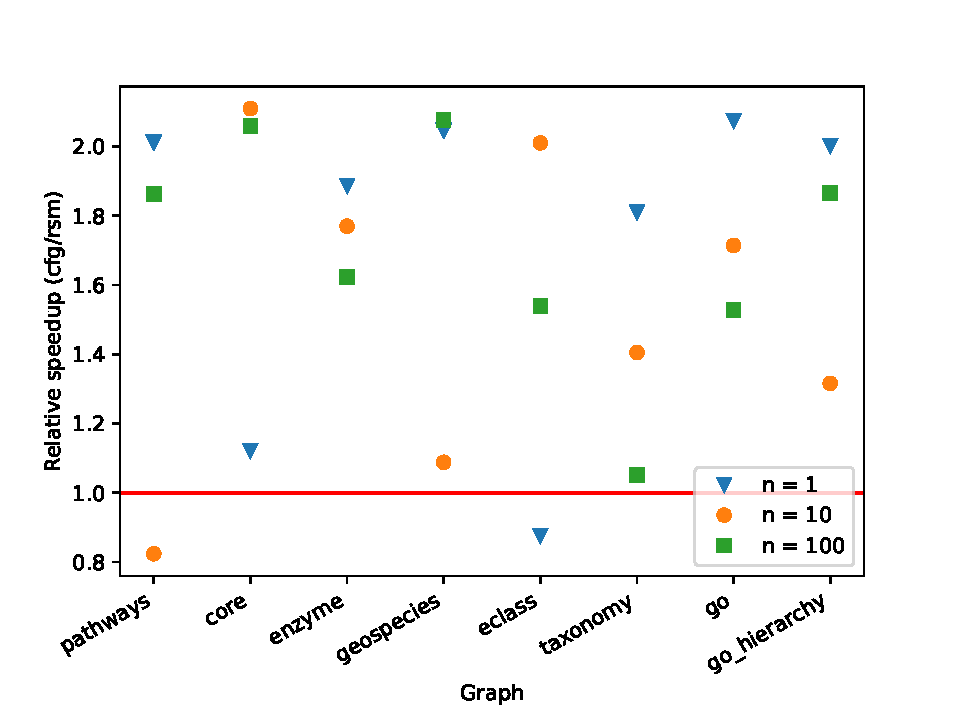
\includegraphics[width=0.49\textwidth]{pictures/g1_kotgll_result.pdf}
    %\caption{ $G_1$ query}            
    %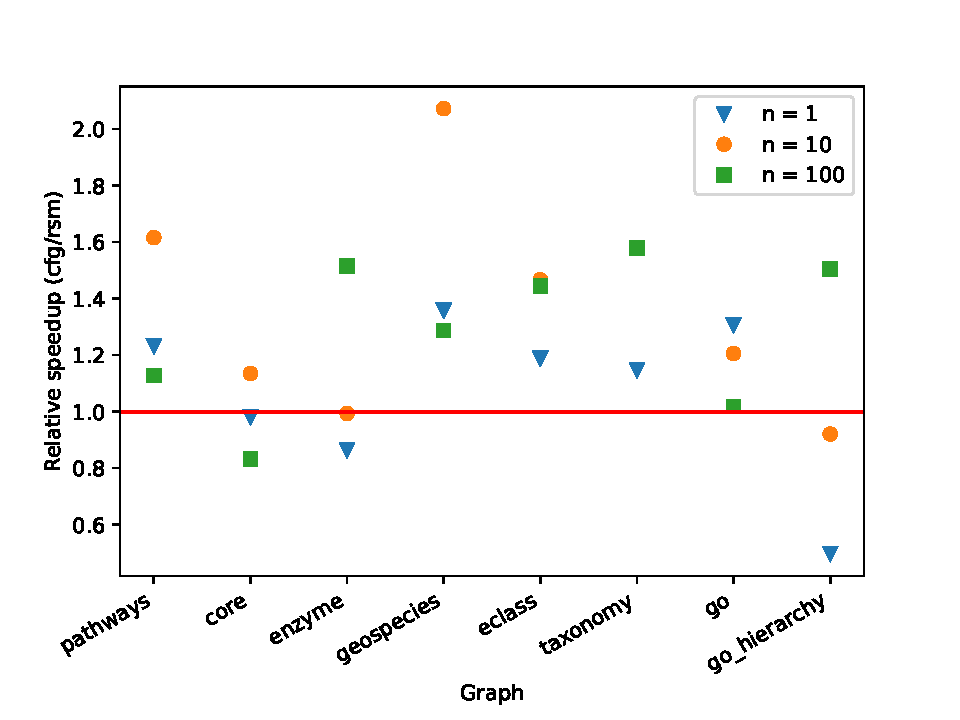
\includegraphics[width=0.3\textwidth]{pictures/g2_kotgll_result.pdf}
    %\caption{$G_2$ query}        
    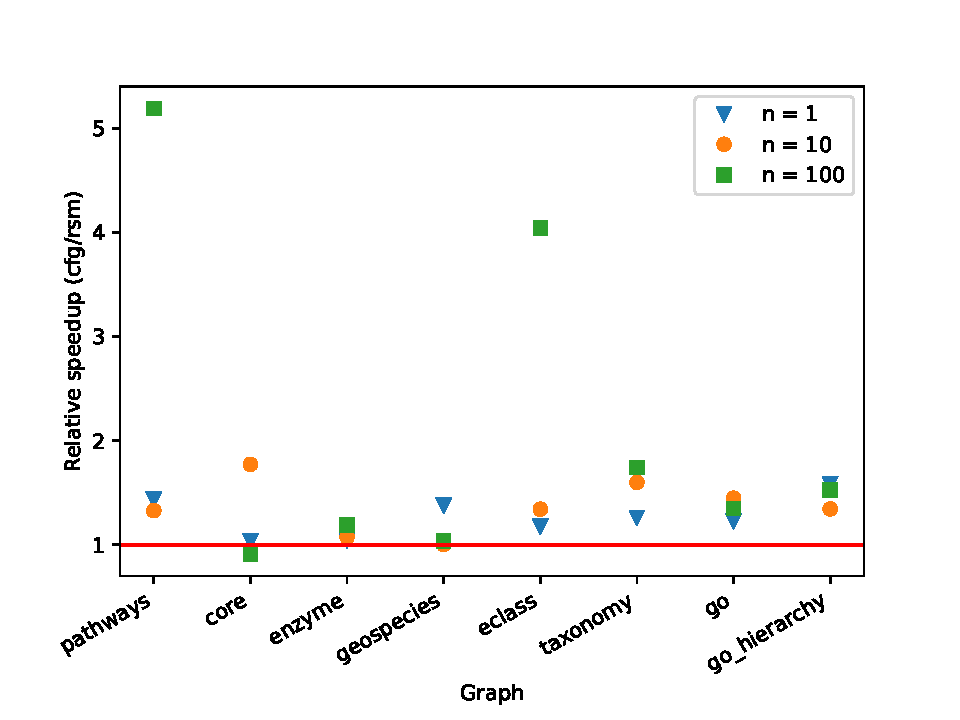
\includegraphics[width=0.49\textwidth]{pictures/geo_kotgll_result.pdf}
    %\caption{$Geo$ query}
  \end{center}
\end{frame}


\begin{frame}[fragile] \frametitle{Multiple sources CFPQ reachability results for queries related to RDF analysis}
  \begin{center}        
    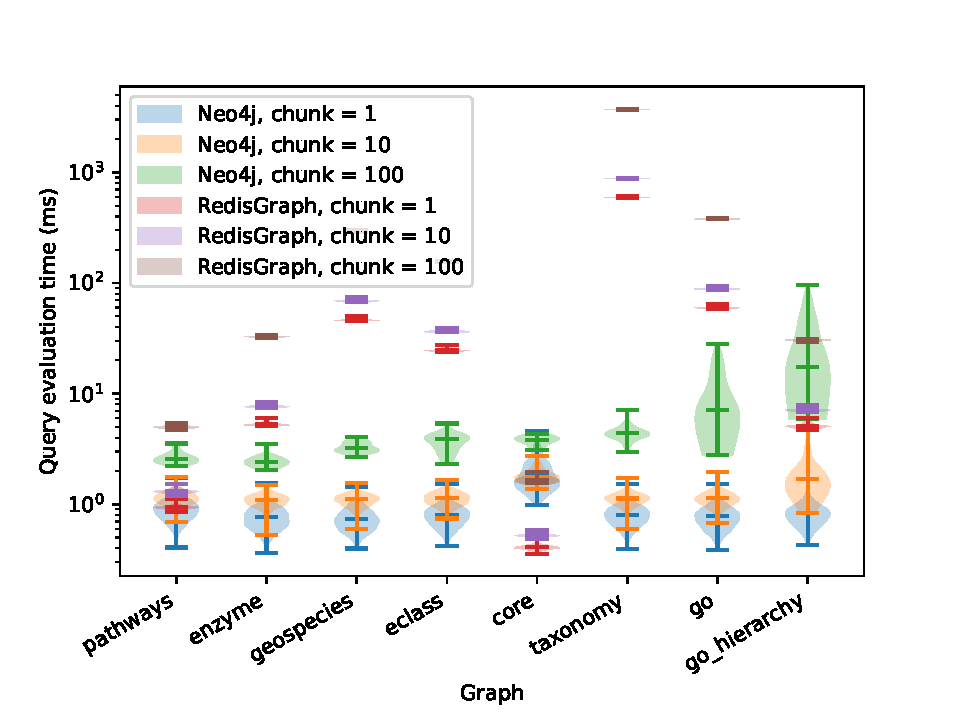
\includegraphics[width=0.49\textwidth]{pictures/g1_result.pdf}
    %\caption{ $G_1$ query}            
    %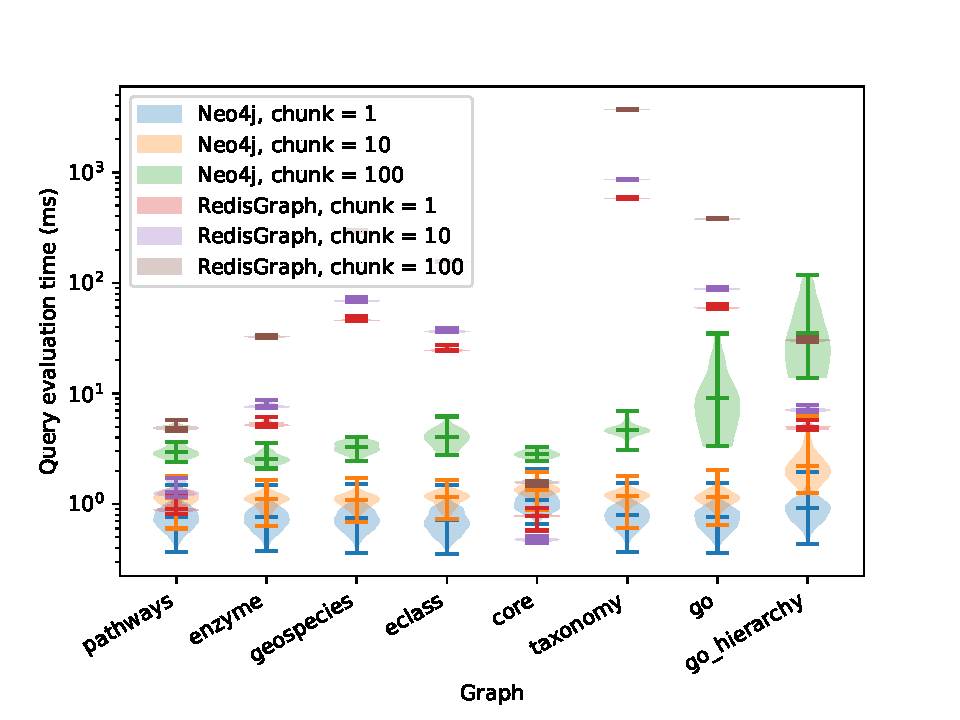
\includegraphics[width=0.3\textwidth]{pictures/g2_result.pdf}
    %\caption{$G_2$ query}        
    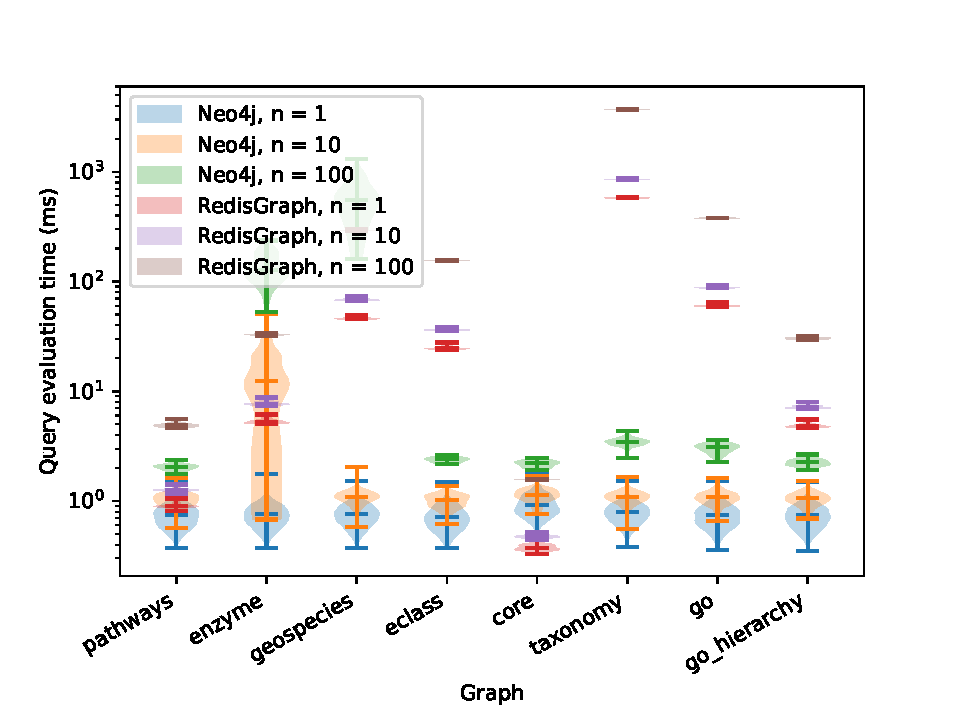
\includegraphics[width=0.49\textwidth]{pictures/geo_result.pdf}
    %\caption{$Geo$ query}
  \end{center}
\end{frame}

\begin{frame}[fragile] \frametitle{Multiple source RPQ reachability results for queries related to RDF analysis and respective query (native solution failed with OOM on last two graphs)}
  \begin{center}        
    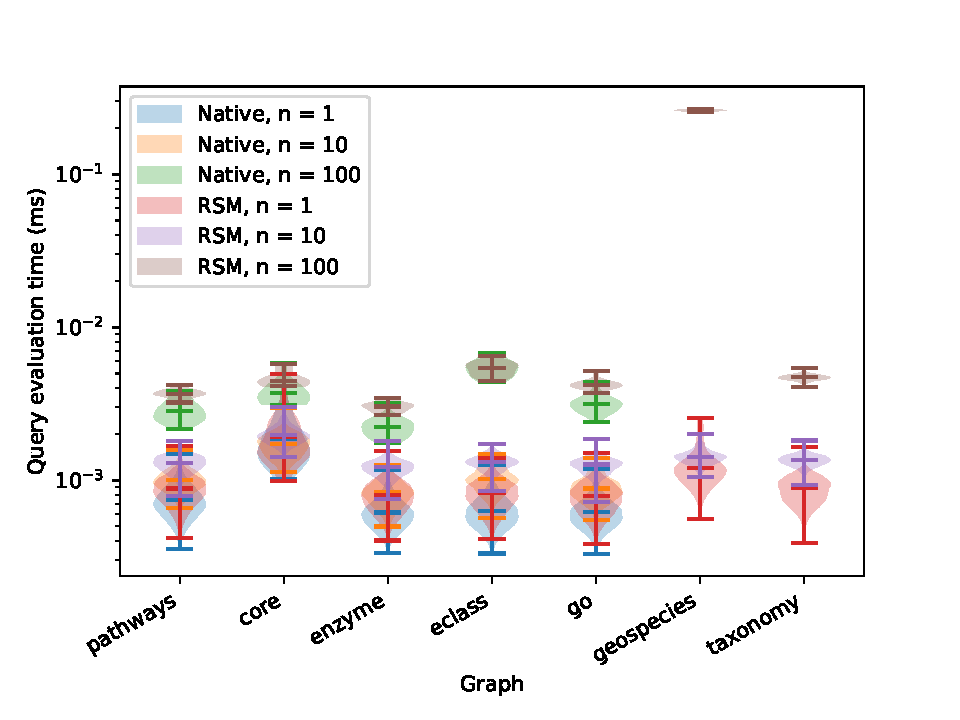
\includegraphics[width=0.49\textwidth]{pictures/reg1_rpq_result.pdf}
    %\caption{ $G_1$ query}            
    %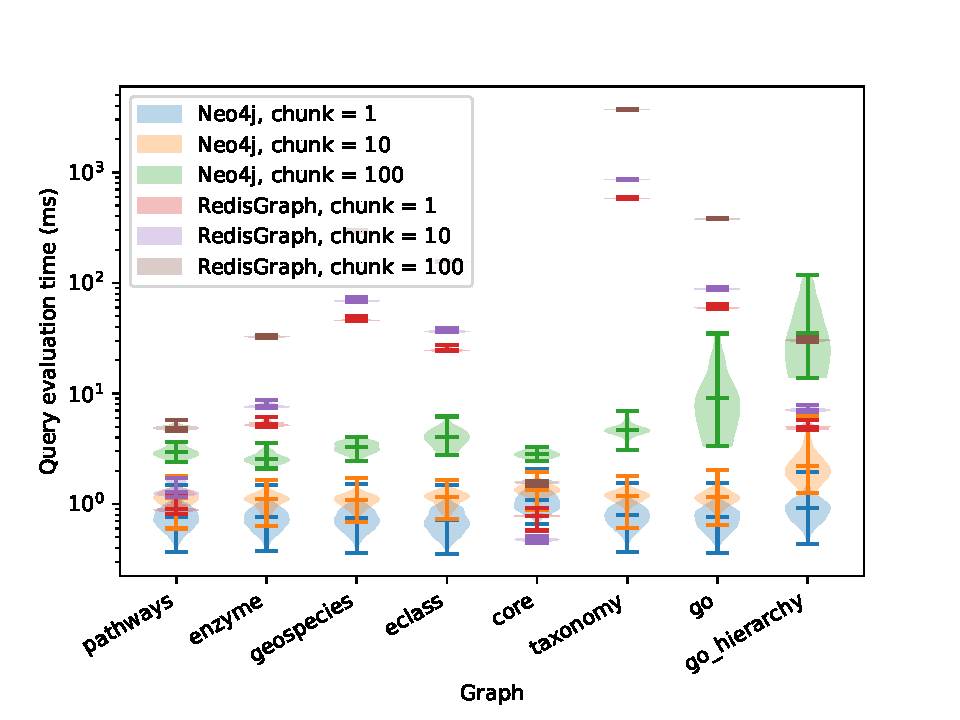
\includegraphics[width=0.3\textwidth]{pictures/g2_result.pdf}
    %\caption{$G_2$ query}        
    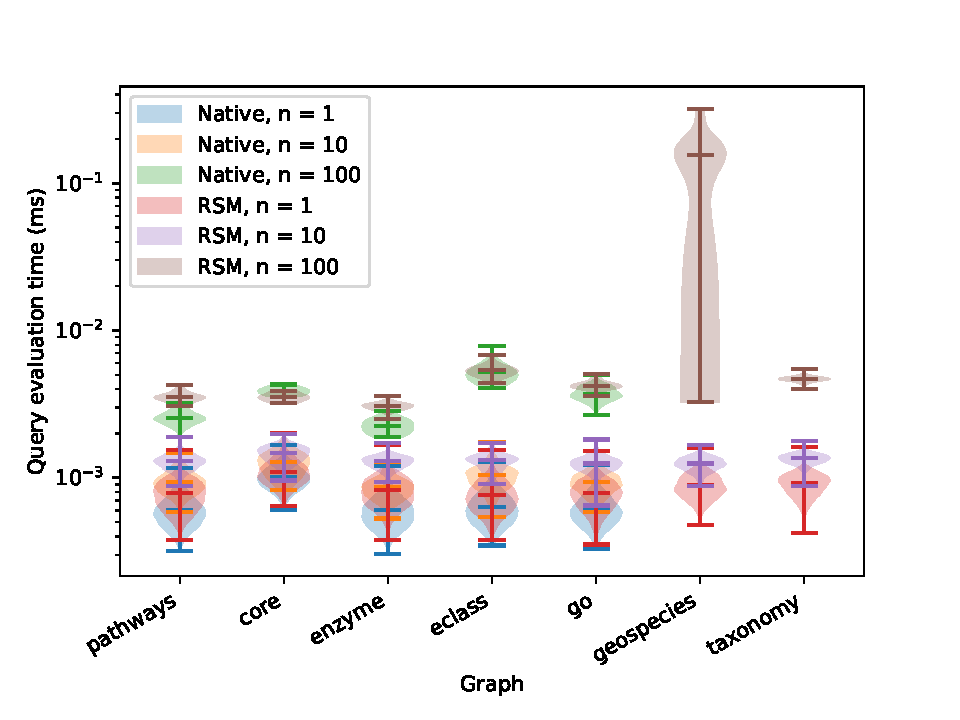
\includegraphics[width=0.49\textwidth]{pictures/reg2_rpq_result.pdf}
    %\caption{$Geo$ query}
  \end{center}
\end{frame}

\begin{frame}[fragile] \frametitle{Conclusion}
  \begin{itemize}
      \item Full-stack support for CFPQ in real-world applications which use RedisGraph database with Cypher query language
      \begin{itemize}
         \item No more context-free grammars
         \item No more custom graph formats and storages
      \end{itemize}
      \item Reasonable performance of context-free path queries
      \begin{itemize}
         \item Multiple-source scenario
         \item Space-time ratio can be tuned
      \end{itemize}
      \item Context-free path queries can be used in applications with well-established tools
  \end{itemize}
\end{frame}



\begin{frame}[fragile] \frametitle{Future Research}
  \begin{itemize}
    \item Mechanization of Cypher semantics in Coq
    \begin{itemize}
      \item Semantics which includes path patterns
      \item Goal: prove correctness of translation to linear algebra
    \end{itemize}
    \pause
    \item Integration of tensor-based CFPQ algorithm\footnote<.(1)->{Egor Orachev, Ilya Epelbaum, R. Azimov and S. Grigorev. 2020. Context-Free Path Querying by Kronecker Product.} to RedisGraph
    \begin{itemize}
      \item The algorithm constructs paths, not only reachability facts
      \item The algorithm should be modified to get multiple-source version
    \end{itemize}
    \pause
    \item Detailed evaluation
    \begin{itemize}
      \item Include more graphs and queries, including RPQs
      \item Evaluate the scalability of the solution
      \item Compare with other graph query engines
    \end{itemize}
  \end{itemize}
\end{frame}

\begin{frame}
\frametitle{Contact Information}
\begin{minipage}[t]{0.8\textwidth}
\begin{itemize}
  \item Try it out (Docker image with extended RedisGraph): \url{https://hub.docker.com/r/simpletondl/redisgraph}
  \item RedisGraph extended with CFPQ: \url{https://github.com/YaccConstructor/RedisGraph}
  \item Cypher parser extended with path patterns: \url{https://github.com/YaccConstructor/libcypher-parser}

  \vspace{0.5cm}
  \pause
  \item Semyon Grigorev: \href{mailto:s.v.grigoriev@spbu.ru}{s.v.grigoriev@spbu.ru}
  \item Arseniy Terekhov: \href{mailto:simpletondl@yandex.ru}{simpletondl@yandex.ru}
  \item Vlada Pogozhelskaya: \href{mailto:pogozhelskaya@gmail.com}{pogozhelskaya@gmail.com}
  \item Vadim Abzalov: \href{mailto:vadim.i.abzalov@gmail.com}{vadim.i.abzalov@gmail.com}
  \item Timur Zinnatulin: \href{mailto:teemychteemych@gmail.com}{teemychteemych@gmail.com}
\end{itemize}
\end{minipage}~
\begin{minipage}[t]{0.19\textwidth}
\pause
\vspace{2.5cm}
\center{\huge{Thanks!}}
\end{minipage}
\end{frame}
\end{document}
